\documentclass[12pt]{article} 
\usepackage[brazil]{babel} %hifenização em português do brasil
%\usepackage[portuguese]{babel}
\usepackage{gensymb}
\usepackage[hidelinks]{hyperref}
\usepackage[T1]{fontenc} % caracteres com acentos são considerados um bloco só
\usepackage{graphicx}
\usepackage{ae} %arruma a fonte quando usa o pacote acima
\usepackage[utf8]{inputenc}
\usepackage{makeidx}
\usepackage{graphicx}%Para inserir figuras

\usepackage{cite}

\begin{document} % Aqui começa o documento
\title{Implementação \textit{system calls} no kernel linux V. 4.13.12\vspace{3.5cm}} % título

\author{
	João Paulo de Oliveira
	\texttt{joaopaulodeoliveira123@gmail.com}
	\and
	Lucas Rossi Rabelo
	\texttt{lucasrossi98@hotmail.com}
	\and		
	Matheus Pimenta Reis
	\texttt{matheuspr96@hotmail.com}
	\vspace*{9cm}
}

\maketitle

\tableofcontents
\pagebreak
\section{Introdução}
Este relatório visa mostrar o processo de criação de uma system call para o sistema Linux cujo a função da mesma é obter:

\begin{itemize}

\item O tempo na qual um processo passou executando na CPU;
\item Quantas vezes um processo passou pela CPU;
\item O tempo desde a criação de um processo até o momento de execução da system call(Tempo de vida do processo).

\end{itemize}

O parâmetro necessário para obter tais informações, é o PID de um processo (Process Identifier ou Identificador do Processo).

Foi utilizada como base para a criação dessa system call, a versão 14.13.12 do kernel do Linux.

\section{Implementação \textbf{System Calls} no Linux}
As \textit{System Calls} fazem o interfaceamento entre o hardware e os processo do espaço de usuário, elas também servem para três propósitos principais:
\begin{enumerate}
	\item Provém abstração com o hardware para que o usuário tenha um maior rendimento. Por exemplo, o usuário não se preocupa com o tipo de partição em que ele lerá um arquivo;
	\item As \textit{system calls} garantem a segurança e estabilidade para que um usuário relativamente leigo possa ter um alto rendimento com gerência de permissão, usuários e outros critérios de gerência do kernel;
	\item Uma camada entre espaço de usuário e o resto do sistema permite fornece o sistema virtualizado para os processos.
\end{enumerate}
	As chamadas syscalls em linux são, na maioria dos casos, acessadas pelas funções definidas na C library. As syscalls em si retornam um valor do tipo long4 que, quando negativo, em geral, denota um erro, já o retorno com valor zero (nem sempre) é um sinal de sucesso. A C library, quando uma \textit{system call} retorna um erro, ela grava o código desse erro na variável global errno, que pode ser ser traduzida para um texto que fala sobre o erro através de funções de biblioteca.
	
	Para a implementação de uma \textit{system call} deve-se ter acesso ao código do kernel do sistema operacional para tanto, foi escolhido o kernel Linux que é open source.
\setcounter{secnumdepth}{-1}

\subsection{Download do Kernel}
Por ser open source, o código fonte do kernel do Linux é mantido online para livre acesso no GitHub(\url{https://github.com/torvalds/linux}), e também em The Linux Kernel Archives (\url{https://www.kernel.org/}) em várias versões e formatos de arquivos(compactados). A versão mais recente dado a data de início do TCD foi a versão \textbf{14.13.12}.
de gerência do kernel.
	A Free Software Foundation mantém, gerencia e presta suporte para o The Linux Kernel Archives.O donwnload do kernel pode ser feito facilmente, além de outras funções com perguntas frequentes, download de versões em teste (beta) para ser compilado em qualquer distribuição linux ou em outras plataformas que suportam o kernel.
	\vspace*{2cm}
	 Como pode ser visto na imagem abaixo:
\begin{figure}[!h]
	\centering
	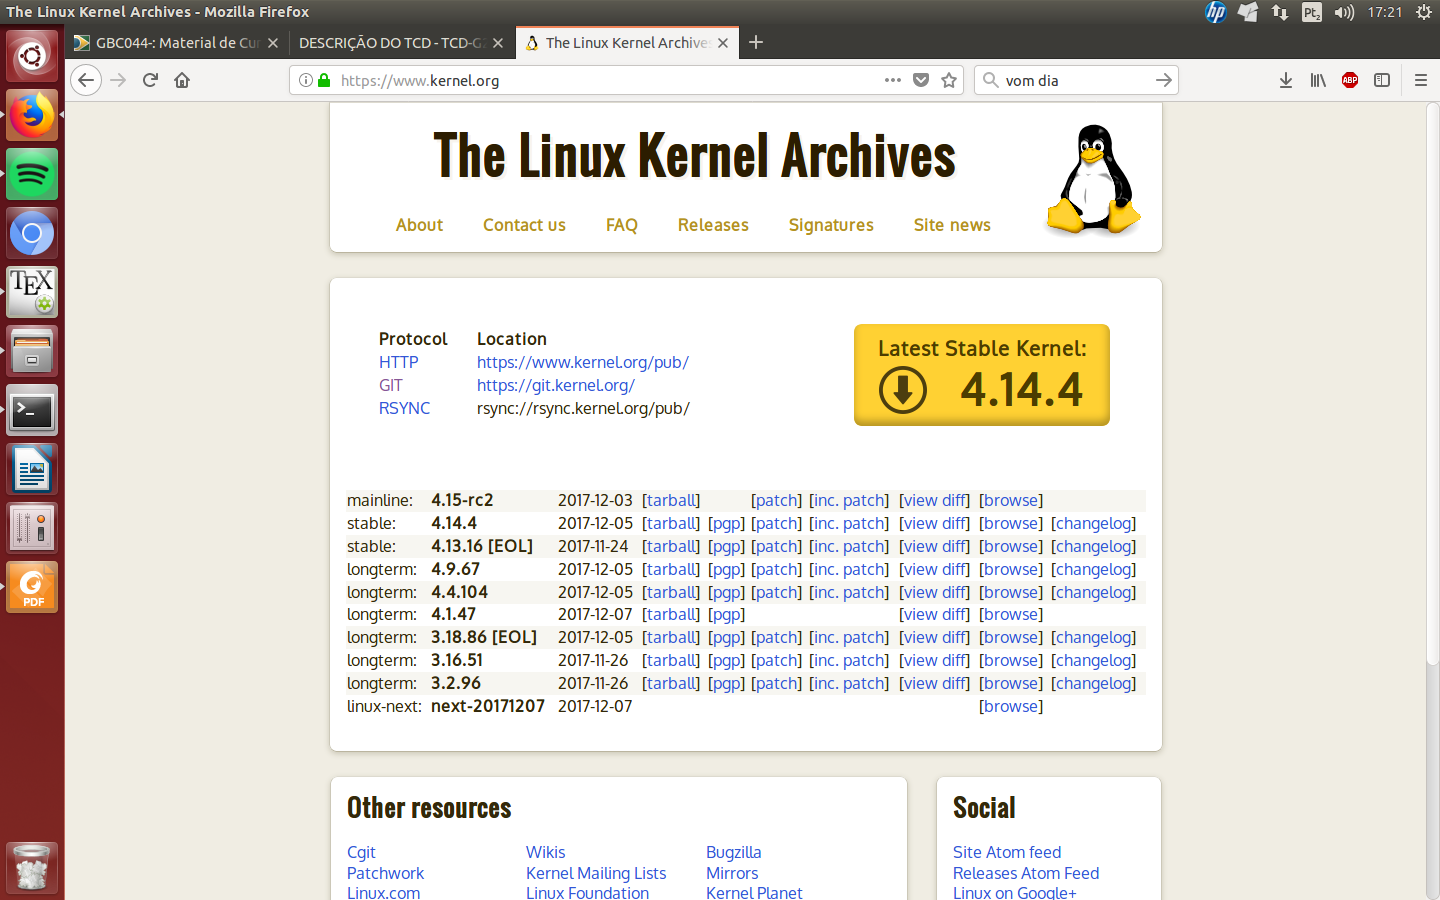
\includegraphics[scale=0.2]{imagens/kernelorg.png}
	\caption{The Linux Kernel Archives: Local de download do Kernel}
	\label{kernelorg}
\end{figure}

\subsection{Compilação do kernel}
	Nesta seção vamos compilar o Kernel que previamente fizemos o Download para trabalhar com ele e assim poder cria nossas System Calls.
	Primeiramente precisamos instalar na nossa maquina um conjunto de ferramentas que nos permitirá compilar nosso kernel, basta abrir seu terminal e digitar o seguinte comando:\newline
	\verb!sudo apt-­get install libncurses5­dev gcc make git exuberant­ctags! 
	\newline
	Criamos uma pasta no nosso espaço de trabalho, posteriormente extraimos todo o conteudo do Kernel com o seguinte comando:\newline \verb!tar xvf linux­­*.tar.xz! \newline onde * é a versão do kernel que acabamos de fazer o download, neste caso usamos linux-12.13.12, então ficou\newline
	\verb!tar xvf linux­3.17.1.tar.xz!\newline
	A seguir abrimos nossa pasta pelo terminal e acessamos onde está o kernel, fazendo uso do comando cd, que permite acessar um diretório.

	Agora iremos compilar nosso kernel completamente, para isso basta usar o comando make, porém existe algumas opções bem úteis para agilizar o processo para isso usamos: \newline
	\verb!make -­j4 CONFIG_LOCALVERSION="tutorial".! \newline
	Ao usar o -j4 dizemos que o processo pode usar quantos processadores estejam disponiveis, no caso do exemplo saõ 4, ou seja, a maquina usada possui 4 processadores para realizar a tarefa, se sua maquina possuir 6, 8, etc você pode substituir pelo número de processadores da sua maquina,ou seja, jX, sendo x o número de processadores da maquina, vale resaltar se existe a necessidade de usar a máquina durante o processo é recomendavel deixar ao menos 1 processador para realizar  ativades. Já o "tutorial" será o nome atribuido ao kernel, que receberá após ser compilado e	que será acessado quando estiver iniciando o ubuntu, pode-se alterar para o nome desejado e fica entre "" ,pois é um conjunto de caracteres, este processo pode demorar ,pois é um processo extremadamente grande, irá depender também da velocidade de processamento da máquina, em testes feitos normalmente demorou entre 2 a 4 horas usando 4 processadores.
	\newline
	Quando por fim a compilação acabar precisa-se substituir o kernel para assim que todas as modificações que seram feitas posteriormente possam ser carregadas com o sistema. Para isso abrir o terminal digir-se na pasta anteriormente criada conforme a imagem anterior, e proseguimos com os seguintes comandos: \newline
	\verb"make modules" \newline
	\verb"sudo make modules_install"\newline
	E por fim instala-se o novo kernel, este comando instala o Kernel, gera a imagem, copia os arquivos para o diretório /boot e atualiza o gerenciador de boot.\newline
	\verb"sudo make install" \newline
	Agora está tudo pronto para acessar o novo kernel usamos terminal com comando:\newline
	\verb"reboot" \newline
	
	Quando estiver na opção de escolher o Sistema Operacional basta acessar opções avançadas do ubuntu e selecionar o kernel, que estará identificado pelo nome inserido no começo, vale resaltar que quando você selecionar o kernel uma vez não é necessário selecionar-lo toda vez que der boot, a máquna carrega o ultimo kernel instalado.
	
\subsection{Criação da System Call}
A \textit{system call} foi criada dentro na pasta kernel no diretório principal deixando o arquivo  scall.c nessa pasta. Após isso foi adicionado o arquivo objeto no arquivo de \textit{makefile} como descrito no tutorial, dessa forma, foi encontrada no arquivo \textit{syscall\_64.tbl} na forma\cite{rubini2001linux} \newline

\textbf{333	common	scall			sys\_det}
\newline
Assim a função pode ser chamada pela função \textit{\textbf{syscall(333)}} presente na \textit{unistd.h}. Por fim, foi adicionado o cabeçalho da função no arquivo \textit{syscall.h}. Depois disso foi compilado o kernel seguindo o tutorial proposto\cite{scall}. 
\\ \newline
\scriptsize{\textbf{unsigned long copy\_to\_user(void \_user *to, const void *from, unsigned long n)};}
\newline
\normalsize
	
Vejamos agora o código do kernel utilizado para:

\subsubsection{Tempo na CPU}
	Como primeira tentativa para obter o tempo de CPU de um processo, acessamos a variável \textit{sum\_exec\_runtime} na estrutura \textit{task\_cputime} \cite{freeelc}, com base nos comentários da estrutura, concluímos que tal variável era o que desejávamos como segue na figura 2: %fazer um hiperlink

\begin{figure}[!htb]
	\centering
	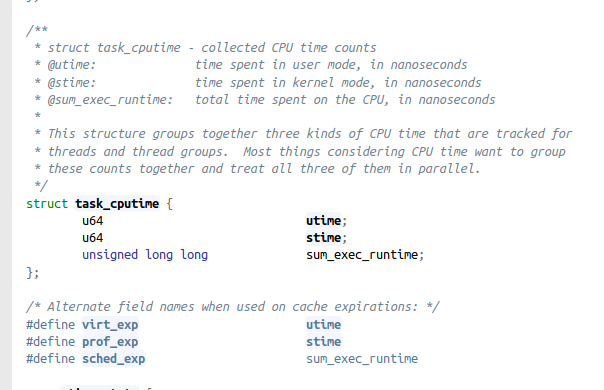
\includegraphics[scale=0.5]{imagens/img1.png}
	\caption{Estrutura task\_cputime}
	\label{taskcputime}
\end{figure}

	No entanto, com a tentativa não obtivemos o resultado esperado.
como segunda tentativa, encontramos uma função chamada get\_sum\_exec\_runtime. A partir de ai decidimos usar o que a função fornece, ou seja, chamar direto na propia task o desejado usando esse "su" que posteriormente seria a shed\_entity como segue a imagem:
 
\begin{figure}[!htb]
	\centering
	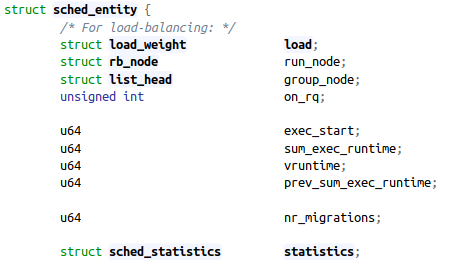
\includegraphics[scale=0.6]{imagens/img2.png}
	\caption{Parte da estrutura sched\_entity}
	\label{schedentity}
\end{figure}

	Que é o resultado que procurávamos, decidimos usar direto pois chamar uma função pode ser menos eficiente que chama-la na propia task\_struct assim obtemos em nano-segundos o tempo que o processo passou pela CPU.

\subsubsection{Tempo de vida do processo}
O tempo de vida do processo não pode ser extraído diretamente, assim a estratégia adotada foi usar a  variável interna à \textit{task\_struck}, a \textit{start\_time} presente na \textit{shed.h}, que é o tempo em nanosegundos contando apartir do boot da máquina (Monotic) \cite{robertlinux}
 \begin{figure}[!htb]
	\centering
	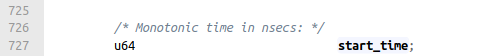
\includegraphics{imagens/start.png} 
	\caption{start\_time: Tempo de vida do processo em nanosegundos contando apartir do boot}
	\label{start}
\end{figure}
A outra variável usada foi a função  \textbf{ktime\_get\_boottime()} presente em \textit{linux/timekeeping.h}. Essa função retorna, intuitivamente, o \textit{boot time} que é o tempo em que a máquina está ligada, desde de o boot até o momento atual. Tendo essas duas variáveis, a \textit{start\_time} foi subtraída do retorno da função \textbf{ktime\_get\_boottime()}, como se segue na figura. Assim foi possível obter o tempo de vida do processo. 
 \begin{figure}[!htb]
	\centering
	
\includegraphics{imagens/life.png} 
	\caption{Tempo de vida do processo em nanosegundos presente na system call}
	\label{life}
\end{figure}

\subsubsection{N$^{\circ}$  de vezes que o processo passou pela CPU}
	Verificando a task\_struct percebemos que tinha uma estrutura que nos auxiliaria chamada shed\_info como segue na figura 5:
 
 \begin{figure}[!htb]
	\centering
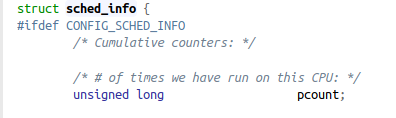
\includegraphics[scale=0.7]{imagens/shed_info.png} 
	\caption{Sched\_info}
	\label{schedinf}
\end{figure}	

 	basta retornar o pcount que obteremos o resultado desejado
 \pagebreak
 
\subsubsection{Retornar -1 caso o processo não exista}
A função \textit{pid\_task} retorna um ponteiro para \textit{task\_struct} dado um PID caso o PID seja zero ou ele não exista, a função retorna NULL\cite{getpid}.

\begin{figure}[!htb]
	\centering
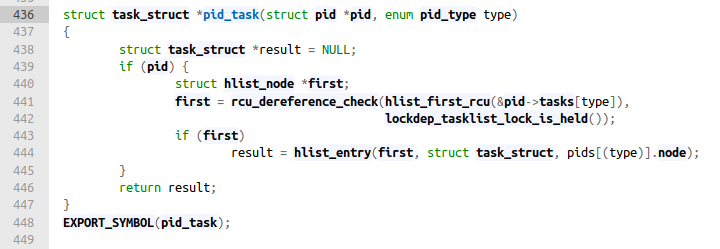
\includegraphics[scale=0.5]{imagens/pid.png} 
	\caption{Estrutura da função que retorna um ponteiro para \textit{tas\_struct} dado um PID}
\end{figure}

Assim, na \textit{system call} foi colocada uma condição na qual, caso a função retorne NULL, a \textit{system call} retornará -1 em todas as variáveis de retorno.
\pagebreak
\section{Código da system call}
	Segue o código:

\begin{figure}[!htb]
	\centering
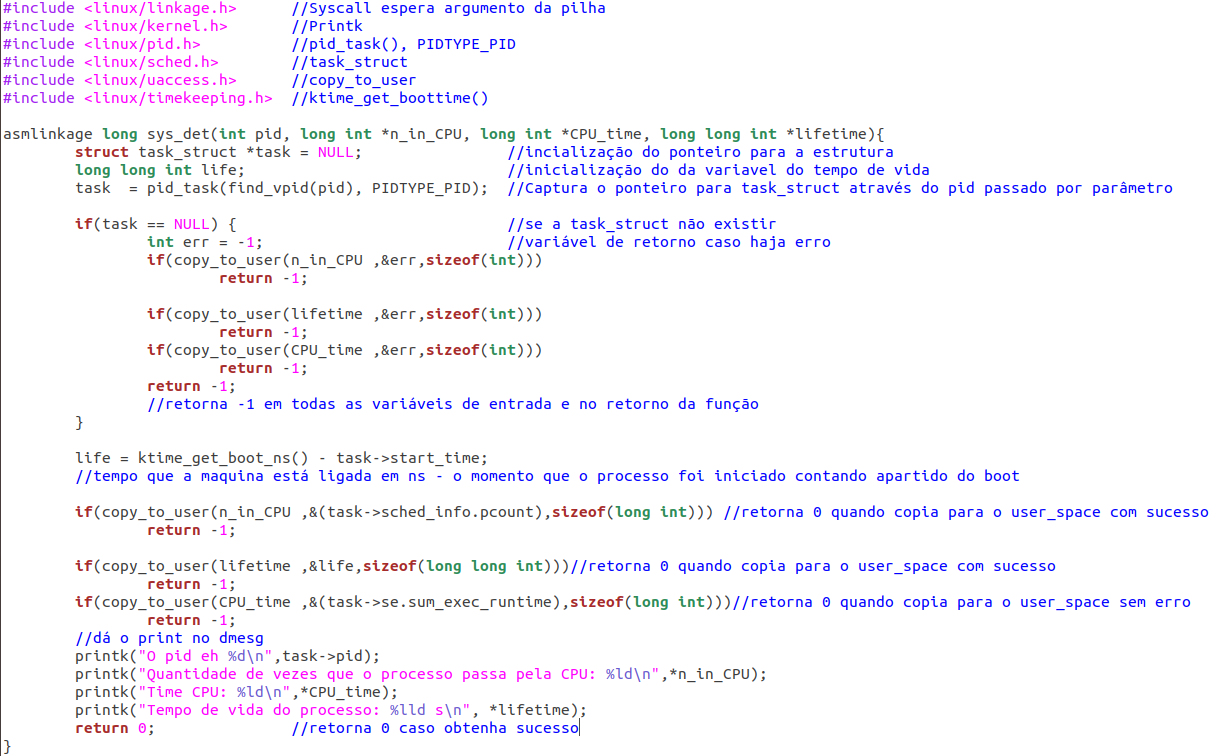
\includegraphics[scale=0.5]{imagens/codsys.png} 
	\caption{Código da system call}
\end{figure}
	
	Foi usada também a função copy\_to\_user para copiar um bloco de dados do kernel para o espaço de usuário para que a função possa retornar por parâmetro
 \pagebreak
 
\section{Compilação parcial do Kernel}
	Agora basta compilar nossa system call porém, diferente da primeira vez vamos fazer uma compilação parcial do kernel, assim todas nossas alterações feita na system call seram carregadas para isso usamos o comando: \newline
	\verb"make bzImage" \newline
após usar este comando basta carregar e instalar os modulos com os seguintes comandos:\newline
	\verb"make modules" \newline
	\verb"sudo make modules_install" \newline
	\verb"sudo make install" \newline
	
	Agora nossa system call está pronta basta reiniciar nossa máquina e estar nossa system call.
 
\section{Programa usuário da system call}
\begin{figure}[!htb]
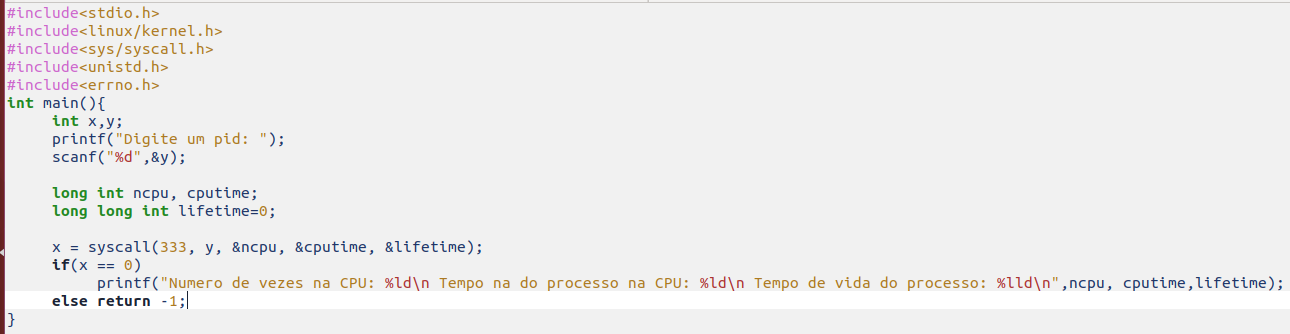
\includegraphics[scale=0.37]{imagens/cod.png} 
	\caption{Código para chamar system call}
\end{figure}

	Basta agora compilar nosso programa no nível de usuário e testar nossa system call e conferir os resultados!

\pagebreak	
	
\section{Conclusão}
Algumas das principais dificuldades que foram encontradas durante a execução deste trabalho foram:

\begin{itemize}

\item O tempo necessário para compilar o kernel;
\item Algumas restrições do próprio kernel, como por exemplo o fato de não poder utilizar o tipo float;
\item Desconhecimento das funções do kernel;
\item A constante atualização das versões do kernel.

Embora tenhamos tido algumas dificuldades, a execução desse trabalho mostrou-se gratificante, pois até então, nunca tivemos a necessidade de programar dentro do kernel de um sistema operacional, porém, essa experiência além de nos possibilitar adquirir um conhecimento maior sobre o funcionamento do kernel de um SO, também nos possibilitou evoluir nossos conhecimentos em programação devido a necessidade de pesquisar sobre outros tipos de dados e outras funções que até então, nunca havíamos utilizado ou sequer ouvido falar. 

\end{itemize}	
	
 \pagebreak

\bibliographystyle{abbrv}
\bibliography{tutorial}

\end{document}
